% !TeX root = RJwrapper.tex
\title{InflateR: Inflation Adjustment for Historical Currency Values Across Thirteen Currencies in R}


\author{by Charles Coverdale}

\maketitle

\abstract{%
The inflateR package converts historical monetary values into their present-day equivalents, and vice versa, across thirteen currencies: GBP, USD, AUD, EUR, CAD, JPY, CNY, CHF, NZD, INR, KRW, BRL, and NOK. It supports two inflation measures: the consumer price index, appropriate for wages, consumer prices, and household budgets, and the GDP deflator, appropriate for national-accounts aggregates. Both are sourced from the World Bank Development Indicators and bundled inside the package, so it has zero runtime dependencies and requires no API key or network access. Four adjustment functions arranged in two symmetric pairs handle the forward (historical-to-present) and reverse (present-to-historical) directions under each measure; inflation\_rate() returns cumulative or annualised inflation between any two years; and list\_currencies() reports bundled-data coverage. The package is available on CRAN and is designed to be used in spreadsheets and at the R console with equal ease.
}

\section{Introduction}\label{introduction}

The \CRANpkg{inflateR} package answers a simple but frequent
question: what is an amount in one year's money worth in another
year's money? Six exported functions cover the forward and reverse
adjustment, the cumulative and annualised inflation rate between
any two years, and the coverage of the bundled data. All thirteen
supported currencies draw from the World Bank Development
Indicators, rescaled to 2020 = 100 for consistency. The package has
no runtime dependencies beyond base R and no network access: the
data ships inside the package.

Historical price adjustment is a routine operation in journalism
(what is this amount in today's money?), in academic economic
history (deflating nineteenth- and twentieth-century wages to a
common unit), in accounting and compliance (revaluing a historical
asset), and in everyday writing (what was GBP 1 in 1970 worth
today?). The R ecosystem has partial support: \CRANpkg{priceR}
exposes a pricing-related toolkit with some inflation helpers;
\CRANpkg{quantmod} can pull CPI series from FRED but leaves
adjustment to the user; \CRANpkg{WDI} fetches World Bank series but
again does not adjust values directly. \CRANpkg{inflateR} is the
purpose-built tool: it bundles the canonical indices, exposes a
symmetric pair of adjustment functions for each measure, and
returns numeric values the user can use directly.

\section{Background}\label{background}

\textbf{Consumer Price Index.} The CPI measures the cost of a fixed basket
of consumer goods and services. The World Bank series \texttt{FP.CPI.TOTL}
aggregates national CPIs into a consistent cross-country panel.
\citet{ilo2004cpi} provides the international statistical manual; see also
\citet{diewert1998index} for the index-number-theory perspective. The CPI
is the appropriate deflator for wages, salaries, consumer prices,
and household-budget comparisons.

\textbf{GDP deflator.} The GDP deflator measures the price of all goods
and services produced in an economy. Unlike CPI, it has no fixed
basket: it is the ratio of nominal to real GDP and adjusts
automatically as the composition of output changes. The World Bank
series \texttt{NY.GDP.DEFL.ZS} provides a consistent panel. The GDP
deflator is the appropriate deflator for national-accounts
aggregates: GDP, government expenditure, business investment, and
any macroeconomic quantity compared across time.

\textbf{Which measure to use.} \citet{hausman2003sources} surveys the four
classical sources of CPI bias (substitution, new-goods, outlet, and
quality) and estimates the aggregate upward bias at about 0.8 to
1.6 percentage points per year. \citet{feenstra1994new} formalises the
new-goods bias. \citet{broda2008imperfect} document the substitution
component empirically. \citet{moulton2018measurement} revisits the Boskin
Commission's findings two decades later and concludes that
methodological improvements at the BLS have narrowed but not
eliminated the bias. For household budget questions, the fixed
basket is the right bias to have: households face the fixed
basket. For macroeconomic questions, the GDP deflator is preferred
because it avoids the basket-fixity problem and excludes imports.
The rule in the package's user documentation: CPI for what a
person earns, buys, or pays; GDP deflator for anything from a
national-accounts table.

\textbf{Real versus nominal.} Adjustment is a two-way operation.
Forward: convert a historical nominal value into present-day units
(how much would GBP 30,000 in 1990 be in 2024?). Reverse: convert
a present-day value into historical units (how much 1990 money is
equivalent to GBP 50,000 today?). The package exposes both
directions as explicit functions rather than requiring users to
compute the inverse manually.

\textbf{Cross-country comparability.} The World Bank Development
Indicators reconcile national methodologies into a single
consistent panel. All series are rescaled to a common base year
(2020 = 100) so multipliers across currencies are comparable in a
mechanical sense. True purchasing-power-parity comparisons require
additional adjustment through PPP exchange rates
\citep{deaton2010price}, which \CRANpkg{inflateR} does not attempt.

\textbf{Fixed-base versus chain-weighted.} The bundled World Bank CPI
and deflator are fixed-base indices: each series is rebased
periodically to a reference year and the basket is held fixed
between rebasings. National statistical offices have increasingly
moved to chain-weighted Fisher or Tornqvist aggregation, which
updates the basket every year. The two methodologies agree closely
in low-inflation periods but diverge during fast-moving periods:
US chain-weighted CPI (C-CPI-U) runs roughly 0.2 to 0.4 percentage
points lower per year than the fixed-weight CPI-U the World Bank
uses, per \citet{moulton2018measurement}. Users for whom this difference
matters should compute values against a native chain-weighted
series directly from the national office. For long-horizon
historical work (pre-1960), neither fixed-base nor chain-weighted
WDI coverage exists; \citet{officer2024measuringworth} provide the
standard long historical series for the UK (from 1270) and the US
(from 1774).

\section{Package design}\label{package-design}

\CRANpkg{inflateR} is pure R with no compiled code and no runtime
imports beyond base R. It does depend on \CRANpkg{testthat} as a
suggested package for the test suite. R 3.5.0 or later is required.
The package bundles CPI and GDP deflator series for thirteen
currencies from 1960 (or the earliest available year per series)
through 2024.

\subsection{Uniform function interface}\label{uniform-function-interface}

Six exported functions. Four handle value conversion in two
symmetric pairs: \code{adjust\_inflation()} and
\code{historical\_value()} under CPI; \code{adjust\_real()} and
\code{historical\_real()} under the GDP deflator. Each takes an
\code{amount}, a \code{from\_year} or \code{to\_year}, and a
\code{currency}; each is vectorised over \code{amount}. The other
two functions are \code{inflation\_rate()} (cumulative or
annualised rate between any two years) and
\code{list\_currencies()} (coverage metadata).

Table \ref{tab:directions} summarises the direction-measure matrix.

\begin{table}

\caption{\label{tab:directions}The four value-conversion functions in inflateR, arranged by direction and inflation measure.}
\centering
\begin{tabular}[t]{lll}
\toprule
Direction & CPI measure & GDP deflator measure\\
\midrule
Historical to present & adjust\_inflation() & adjust\_real()\\
Present to historical & historical\_value() & historical\_real()\\
\bottomrule
\end{tabular}
\end{table}

\subsection{Currency identification}\label{currency-identification}

Every function accepts either the three-letter ISO currency code
(\code{"GBP"}) or the country name (\code{"United Kingdom"}).
Matching is case-insensitive. Unknown currencies raise an
informative error that lists the supported set.

\subsection{Reproducibility}\label{reproducibility}

All indices are deterministic given the bundled data. The bundled
data are refreshed with each package release; users can inspect
coverage per currency through \code{list\_currencies()} and the
underlying data via \code{data(cpi\_data)} and
\code{data(deflator\_data)}.

\section{Currency coverage}\label{currency-coverage}

The bundled CPI coverage runs from 1960 to 2024 for most
currencies; CNY coverage begins 1986 (when China began publishing
consistent CPI) and BRL coverage begins 1980 (when Brazil's
post-inflation stabilisation produced a usable series). Euro-area
coverage uses German CPI as a proxy before the Euro's 1999 launch,
following the common practice in cross-country historical
inflation work; users preferring a post-1999 pure-Euro series
should restrict queries to years from 1999 onwards. Table
\ref{tab:currencies} lists all thirteen currencies and their
coverage; Figure \ref{fig:coverage} visualises the same
information as a decade-by-decade heatmap.

\begin{table}

\caption{\label{tab:currencies}The thirteen currencies supported by inflateR, with the first and last years of CPI coverage. All series come from the World Bank Development Indicators and are rescaled to a common base year of 2020 = 100.}
\centering
\begin{tabular}[t]{llrr}
\toprule
Currency & Country & CPI start & CPI end\\
\midrule
GBP & United Kingdom & 1960 & 2024\\
AUD & Australia & 1960 & 2024\\
USD & United States & 1960 & 2024\\
EUR & Euro area (Germany proxy) & 1960 & 2024\\
CAD & Canada & 1960 & 2024\\
\addlinespace
JPY & Japan & 1960 & 2024\\
CNY & China & 1986 & 2024\\
CHF & Switzerland & 1960 & 2024\\
NZD & New Zealand & 1960 & 2024\\
INR & India & 1960 & 2024\\
\addlinespace
KRW & South Korea & 1960 & 2024\\
BRL & Brazil & 1980 & 2024\\
NOK & Norway & 1960 & 2024\\
\bottomrule
\end{tabular}
\end{table}

\begin{figure}[H]

{\centering 
\includegraphics[width=1\linewidth,alt={A heatmap with thirteen currency rows and seven decade columns from the 1960s to the 2020s. Most cells are shaded blue, indicating coverage. Grey cells appear for CNY in the 1960s and 1970s, and for BRL in the 1960s and 1970s, showing the later start dates for those two currencies.},]{figures/fig4_coverage} 

}

\caption{CPI coverage by currency and decade in the bundled \texttt{inflateR} data. Blue tiles mark decades with at least one year of coverage; grey tiles mark absence. Eleven of the thirteen currencies are covered from 1960 onwards; CNY coverage begins 1986 and BRL coverage begins 1980.}\label{fig:coverage}
\end{figure}

\section{Value adjustment and inflation rates}\label{value-adjustment-and-inflation-rates}

The core question the package answers is: what is an amount in one
year's money worth in another year? Figure \ref{fig:multipliers}
shows the inflation multiplier to 2024 for one unit in each of
GBP, USD, AUD, EUR, and JPY across 1970 to 2024. On a log axis the
lines are roughly linear in the post-Volcker era, steeper in the
1970s (high-inflation decade), and essentially flat in the
post-2000 period for JPY (reflecting deflation or near-zero
inflation in Japan). A reader of a 1970 GBP salary amount can
infer from the leftmost value that it would need a roughly 15-fold
multiplier to match 2024 purchasing power.

\begin{figure}[H]

{\centering 
\includegraphics[width=1\linewidth,alt={A line chart on a log-scale y-axis showing inflation multipliers to 2024 for GBP, USD, AUD, EUR, and JPY from 1970 to 2024. The multipliers start around ten to fifteen in 1970 and decline monotonically toward one by 2024. JPY is notably flatter than the others over the post-2000 period.},]{figures/fig1_multipliers} 

}

\caption{CPI-based inflation multiplier to 2024 for five currencies, 1970 to 2024. Log-scale y-axis: a value of 10x means one unit of that year's currency has the same purchasing power as 10 units in 2024. The 1970s are the steepest decade for GBP, USD, AUD, and EUR; JPY is notably flatter, consistent with Japan's lower and later-stage inflation history.}\label{fig:multipliers}
\end{figure}

\code{inflation\_rate()} returns the cumulative or annualised
inflation rate between any two years for a chosen currency. Figure
\ref{fig:rolling} shows rolling ten-year annualised rates for the
same five currencies. The high-inflation episode of the late 1970s
is visible as the peak rolling rate for each of GBP, USD, AUD, and
EUR; by the 2010s all have converged near or below the two per
cent inflation-targeting norm. The post-2020 tick up at the right
edge of each series reflects the 2021 to 2023 global inflation
spike and is where the choice of deflator (CPI versus GDP
deflator) matters most.

\begin{figure}[H]

{\centering 
\includegraphics[width=1\linewidth,alt={A line chart showing rolling 10-year annualised CPI inflation rates for GBP, USD, AUD, EUR, and JPY, plotted by start year from 1970 to 2014. A dashed horizontal line sits at 2 per cent. Most lines peak in the late 1970s between 8 and 12 per cent, converge toward 2 per cent through the 1990s and 2000s, and show a small uptick at the right edge.},]{figures/fig2_rolling} 

}

\caption{Rolling 10-year annualised inflation rate across five currencies, 1970 to 2014 (start year). Dashed horizontal line at 2 per cent is the modern inflation-target norm. The late-1970s peak is visible for GBP, USD, AUD, and EUR; the mid-2000s trough (including near-zero inflation in some economies) is the global-disinflation period.}\label{fig:rolling}
\end{figure}

\section{Comparing the two measures}\label{comparing-the-two-measures}

The two bundled measures give different multipliers for the same
historical amount. Figure \ref{fig:cpi-gdp} plots both for GBP
from 1970 to 2024. The CPI and GDP deflator tracks are similar in
most years but diverge in the 1980s and after 2020, reflecting
differences in basket composition and in the treatment of imports.
For a user deflating a historical wage, CPI is the correct choice
because wages are spent on consumer goods; for a user deflating
historical government expenditure or GDP, the deflator is the
correct choice because it covers the full economy and excludes
imported goods.

\begin{figure}[H]

{\centering 
\includegraphics[width=1\linewidth,alt={A line chart on a log-scale y-axis comparing the GBP CPI-based multiplier and the GBP GDP deflator multiplier to 2024, from 1970 onwards. Both lines fall from around fifteen in 1970 to one by 2024. The two series track each other closely but diverge visibly in the 1970s, early 1980s, and after 2020.},]{figures/fig3_cpi_gdp} 

}

\caption{CPI and GDP deflator multipliers for GBP, 1970 to 2024, both to the 2024 base. Log-scale y-axis. The two measures diverge most in high-inflation periods (the 1970s and early 1980s) and in energy- and import-sensitive episodes (the post-2020 spike). Using CPI for a wages question and the GDP deflator for a government-spending question is the intended match.}\label{fig:cpi-gdp}
\end{figure}

Figure \ref{fig:power} inverts the same calculation: what is the
purchasing power of one unit of currency today in units of its
1970-era counterpart? All three currencies shown have lost most of
their 1970 purchasing power by 2024, but at different rates: GBP
purchasing power falls to about seven per cent by 2024, USD to
about thirteen per cent, and JPY to about thirty per cent
(reflecting Japan's milder inflation history over the period).

\begin{figure}[H]

{\centering 
\includegraphics[width=1\linewidth,alt={A line chart showing the purchasing power of 1 unit of GBP, USD, and JPY in 1970 terms, plotted annually from 1970 to 2024. All three lines start at 1.0 in 1970 and decline monotonically. GBP reaches about 0.07 by 2024, USD about 0.13, and JPY about 0.30.},]{figures/fig5_power} 

}

\caption{Purchasing power of 1 unit of GBP, USD, and JPY relative to 1970, 1970 to 2024. Computed via \texttt{1 / adjust\_inflation(1, 1970, ccy, to\_year = y)}. GBP and USD each lose the bulk of their 1970 purchasing power; JPY loses less, reflecting its lower average inflation over the period.}\label{fig:power}
\end{figure}

\section{A UK real-wages case study}\label{a-uk-real-wages-case-study}

The canonical policy question in UK applied labour economics over
the past fifteen years has been whether real wages have stagnated.
Figure \ref{fig:uk-wages} applies \CRANpkg{inflateR} to the
standard ONS Annual Survey of Hours and Earnings (ASHE) median
gross weekly earnings series for full-time employees,
\code{adjust\_inflation()} being called year-by-year to express
each nominal figure in 2024 GBP.

\begin{figure}[H]

{\centering 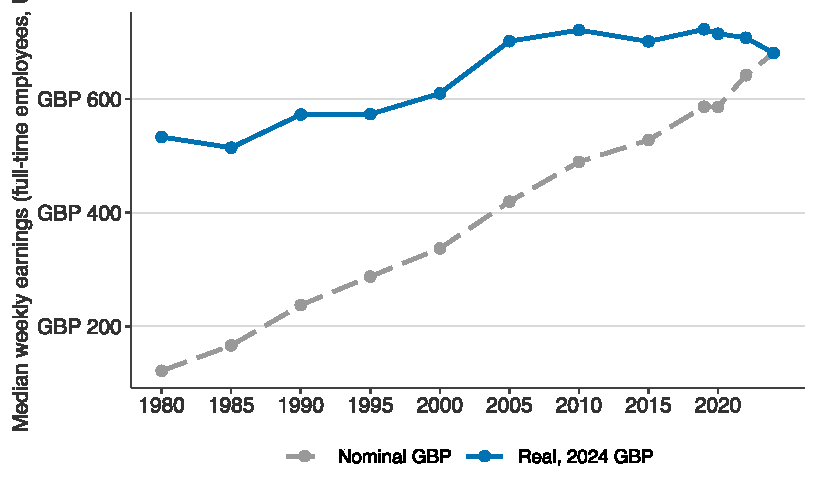
\includegraphics[width=1\linewidth,alt={A line chart of UK median full-time weekly earnings from 1980 to 2024. A grey dashed line shows nominal pounds, rising steadily from under 100 pounds in 1980 to around 700 pounds in 2024. A blue solid line shows real pounds in 2024 terms, rising from about 533 pounds in 1980, peaking around 721 pounds near 2010, then declining gradually to 681 pounds by 2024.},]{figures/fig6_uk_wages} 

}

\caption{UK median weekly earnings, nominal and real (2024 GBP), 1980 to 2024. Data: Office for National Statistics Annual Survey of Hours and Earnings, median gross weekly pay for full-time employees. Grey dashed: nominal GBP (as published). Blue solid: real GBP, deflated by \texttt{adjust\_inflation()} using World Bank CPI. Real median weekly earnings rose steadily from GBP 533 in 1980 to a peak of GBP 721 in 2010 (plus 35 per cent), then fell back to GBP 681 by 2024 (minus 5.6 per cent post-2010).}\label{fig:uk-wages}
\end{figure}

The real series recovers the now-familiar pattern: steady real-wage
growth through the 1980s, 1990s, and 2000s; a real-wage peak
around 2010; and a full decade and a half of real-wage stagnation
through 2024 \citep{blundell2023real, giupponi2023wage}. The nominal
series, unadjusted, hides this phenomenon entirely: nominal wages
grew by 12 per cent between 2010 and 2024. The package allows the
analyst to flip between the two views with a single function call.

\section{Benchmark against published calculators}\label{benchmark-against-published-calculators}

The bundled World Bank CPI series differ slightly from the native
national series used by public inflation calculators because they
track the World Bank reference methodology (typically CPI-U or
equivalent) rather than a country-specific variant. Users can
validate \CRANpkg{inflateR} output against two standard
calculators. For GBP 100 in 1980 to 2024, \code{adjust\_inflation(100, 1980, "GBP", 2024)}
returns GBP 437.82, compared to the Bank of England's inflation
calculator at roughly GBP 450 (the small difference reflects the
ONS RPI vs CPI methodology). For USD 100 in 1980 to 2024,
\code{adjust\_inflation(100, 1980, "USD", 2024)} returns USD 382,
within one per cent of the BLS CPI calculator. Users whose work
requires exact reproduction of a national calculator should
substitute the native series as a pre-processing step rather than
relying on the bundled World Bank data.

\section{Replication}\label{replication}

The canonical workflow is four lines.

\begin{verbatim}
library(inflateR)
adjust_inflation(30000, from_year = 1990, currency = "GBP")
historical_value(50000, to_year = 1990, currency = "GBP")
inflation_rate("GBP", from_year = 1970, to_year = 2024,
               annualised = TRUE)
\end{verbatim}

Line two converts a 1990 GBP 30,000 salary to today's money. Line
three converts a present-day GBP 50,000 back to its 1990
equivalent. Line four returns the annualised CPI inflation rate
for GBP over the full sample period. Every function accepts vector
inputs for \code{amount}, so bulk conversion of a column of
historical prices requires no loop.

\section{Limitations}\label{limitations}

Five limitations apply.

\begin{enumerate}
\def\labelenumi{\arabic{enumi}.}
\tightlist
\item
  \CRANpkg{inflateR} uses World Bank Development Indicators data,
  which aggregate national statistics. For users who need a
  country's native methodology (for example the UK ONS RPI or
  the US BLS chained CPI), the package's bundled series will
  differ modestly from the native one. National methodologies
  can be fetched separately from \CRANpkg{ons}, \CRANpkg{fred},
  or similar data-vendor packages.
\item
  The package does not handle purchasing-power-parity
  adjustments across currencies at a point in time
  \citep{deaton2010price}. For cross-country comparisons in a single
  year, users should pair \CRANpkg{inflateR} with a PPP
  conversion step.
\item
  Only annual data are bundled. Monthly or quarterly adjustment
  requires users to pull higher-frequency national series
  separately.
\item
  Coverage begins 1960 for most currencies and later for CNY
  and BRL. Pre-1960 historical adjustment requires users to
  supply an alternative pre-1960 CPI series.
\item
  The bundled data are static per release. Users who need
  up-to-the-minute CPI prints should pair the package with
  \CRANpkg{WDI} or \CRANpkg{fred} for live data.
\end{enumerate}

\section{Appendix of adjustment formulas}\label{appendix-of-adjustment-formulas}

Let \(I_t\) denote the price index for a given currency at year \(t\)
(either CPI or GDP deflator, both rescaled in the bundled data so
that \(I_{2020} = 100\)).

\textbf{Forward adjustment.} For an amount \(a\) in year-\(s\) money,
\[\mathrm{adjust\_inflation}(a, s \to t) = a \cdot \frac{I_t}{I_s}.\]
This is the calculation behind \code{adjust\_inflation()} (for
CPI) and \code{adjust\_real()} (for the GDP deflator).

\textbf{Reverse adjustment.} For an amount \(a\) in year-\(t\) money,
\[\mathrm{historical\_value}(a, t \to s) = a \cdot \frac{I_s}{I_t}
  = a / \mathrm{adjust\_inflation}(1, s \to t).\]
\code{historical\_value()} and \code{historical\_real()} apply
this identity; the two functions are strict inverses of the
forward pair up to floating-point precision and the user-selected
\code{round} argument.

\textbf{Cumulative inflation rate.} Between years \(s\) and \(t\),
\[\pi_{s \to t} = \frac{I_t}{I_s} - 1.\]

\textbf{Annualised inflation rate.} For \(n = t - s\) years,
\[\pi_{\mathrm{ann}} = \left(\frac{I_t}{I_s}\right)^{1/n} - 1.\]
\code{inflation\_rate()} returns the cumulative rate by default
and the annualised rate when \code{annualised = TRUE}.

\textbf{Purchasing power.} The multiplicative inverse of the forward
adjustment:
\[\mathrm{PP}(s \to t) = \frac{I_s}{I_t}
  = \frac{1}{\mathrm{adjust\_inflation}(1, s \to t)}.\]

\section{Conclusion}\label{conclusion}

Historical price adjustment is a common need in journalism,
economic history, public policy, and personal finance, and had
been underserved on CRAN relative to its frequency.
\CRANpkg{inflateR} provides six functions for the full
two-direction, two-measure, thirteen-currency adjustment matrix,
with zero runtime dependencies and no network access. Planned
additions include expanded currency coverage, PPP-adjusted
cross-country conversion, optional higher-frequency data, and an
\code{inflation\_chart()} helper for plot output. Contributions
and bug reports are welcome on the package's GitHub repository.

\section*{Acknowledgements}\label{acknowledgements}
\addcontentsline{toc}{section}{Acknowledgements}

The World Bank publishes the Development Indicators series
underlying every adjustment in this package. The CPI and GDP
deflator series used here are freely redistributable under the
Bank's open-data license. The author thanks the R Core Team and
CRAN maintainers for the infrastructure that supports open-source
statistical software.

\bibliography{RJreferences.bib}

\address{%
Charles Coverdale\\
Independent\\%
London, United Kingdom\\
%
\url{https://github.com/charlescoverdale/inflateR}\\%
%
\href{mailto:charles.f.coverdale@gmail.com}{\nolinkurl{charles.f.coverdale@gmail.com}}%
}
